\section{Scaling laws: Kaplan et al.}
\label{ch:kaplan}

\newthought{Most of what we now call} ``the LLM playbook'' rests on a single
empirical observation made between 2017 and 2020 and crystallised by
\citet{kaplan2020scaling}. The observation: as you make a transformer
language model bigger, give it more data, and train it longer, its loss
follows a smooth power law in each of those resources. Plotting loss against
any of them on log-log axes gives a \emph{straight line}.

That line is the reason the field collectively decided to spend hundreds of
millions of dollars per training run. Before it, scaling up was speculative.
After it, scaling up was a quantitative bet with predictable payoff.

\subsection{The three power laws}

\citet{kaplan2020scaling} swept seven orders of magnitude of model size and
five of data, training transformers on text. They fit:
\begin{align}
  L(N) &\;\approx\; \left(\frac{N_c}{N}\right)^{\alpha_N},
  & \alpha_N &\;\approx\; 0.076 \\
  L(D) &\;\approx\; \left(\frac{D_c}{D}\right)^{\alpha_D},
  & \alpha_D &\;\approx\; 0.095 \\
  L(C) &\;\approx\; \left(\frac{C_c}{C}\right)^{\alpha_C},
  & \alpha_C &\;\approx\; 0.050,
\end{align}
where \(N\) is non-embedding parameters, \(D\) is dataset tokens, and \(C\)
is training compute in PF-days.\sidenote{Here \(C\) is in \emph{petaflop-days} (PF-days): roughly \(10^{15}\) floating-point operations (FLOPs) at nominal throughput, integrated over one day of training wall-clock (see \citealp{kaplan2020scaling} for conventions). The constants \(N_c, D_c, C_c\) and
exponents \(\alpha_*\) are fitted from the empirical sweeps. They shift
slightly with corpus and architecture but the shape (a power law over
many orders of magnitude) is remarkably stable.} Each holds when the named
resource is the \emph{bottleneck}. When it is not, the loss flattens out
into a regime governed by whatever is the next-tightest constraint.

\subsection{What ``straight on log-log'' actually means}

Take logs of \(L(N) = (N_c/N)^{\alpha_N}\):
\begin{equation}
  \log L \;=\; \alpha_N \log N_c - \alpha_N \log N.
\end{equation}
Plot \(\log L\) against \(\log N\): a line with slope \(-\alpha_N\). For
\(\alpha_N = 0.076\), every \(10\times\) in \(N\) buys roughly an
\(0.076\)-decade fall in loss, i.e.\ about a 16\% reduction in cross-entropy.
That sounds tiny, but it compounds over many orders of
magnitude, and small drops in cross-entropy translate into qualitatively
different model behaviour at the right scale.

\paragraph{Why this is so important.} Most engineering quantities saturate.
Add more cores, you eventually hit Amdahl's law. Add more disk, you eventually
hit network. Power laws don't saturate. They slow. The Kaplan curves told
the field that a model 100$\times$ bigger \emph{will} be measurably better,
and quantified by how much. That is the licence to spend.

\begin{figure}
\centering
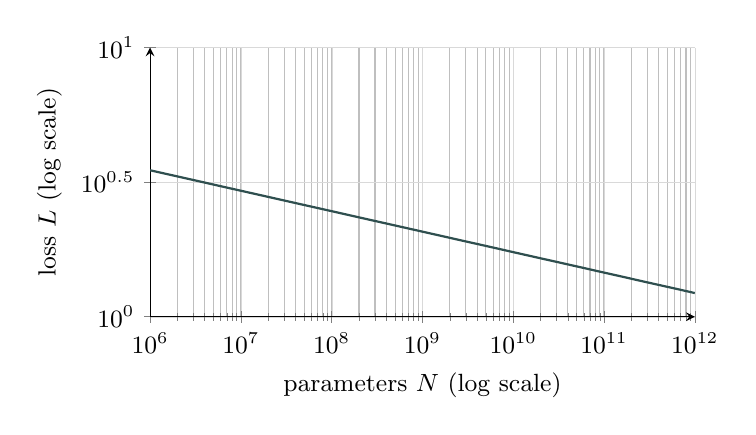
\begin{tikzpicture}
\begin{loglogaxis}[
  width=8.5cm, height=5cm,
  xlabel={parameters \(N\) (log scale)},
  ylabel={loss \(L\) (log scale)},
  xmin=1e6, xmax=1e12,
  ymin=1, ymax=10,
  axis lines=left,
  grid=both,
  major grid style={line width=.1pt, draw=gray!30},
  tick pos=left,
  ticklabel style={font=\small},
  label style={font=\small},
]
  \addplot[domain=1e6:1e12, samples=40, thick, color=DarkSlateGray] {10*x^(-0.076)};
\end{loglogaxis}
\end{tikzpicture}
\caption{The shape of \(L(N)\) on log-log axes. Straight, with slope
\(-\alpha_N\). Same picture for \(L(D)\) and \(L(C)\). Numbers are
illustrative; the point is the geometry.}
\end{figure}

\subsection{Architecture details barely matter (within reason)}

Another result, almost as important as the lines themselves: depth, width,
heads, head dimension, layer normalisation flavour. All of those move the
intercept of the line by a small amount, but not the slope. Within a
generous envelope, what determines loss is total parameter count, not how
those parameters are arranged.

This is why papers comparing two architectures on a single point estimate
of model size are often misleading: the difference between, say, GPT-style
and BERT-style at 350M parameters tells you almost nothing about which would
win at 70B parameters.

\subsection{What Kaplan got slightly wrong}

The original paper recommended that, given a fixed compute budget, you
should make models \emph{larger} faster than you should give them more data.
This was the recipe behind GPT-3 (175B parameters, ${\sim}300$B training
tokens. A token-to-parameter ratio of less than 2). Two years later,
Chinchilla \citep{hoffmann2022training} re-ran the analysis with a wider
sweep and found that the optimal allocation shifts the other way:
parameters and tokens should grow \emph{together}, with a token-to-parameter
ratio of roughly 20.

\paragraph{An illustrative extrapolation.}
The compact toy form
\begin{equation}
  L(N) \;\approx\; L(N_{0})\,\left(\frac{N_{0}}{N}\right)^{\alpha_{N}},
  \quad \alpha_{N} = 0.076,
\end{equation}
anchored to GPT-3 (\(N_{0} \approx 1.75\times 10^{11}\) parameters) with a reported
WebText cross-entropy near \(1.7\)~nats,\sidenote{Actual frontier runs blend many
datasets and recipes; treat \(L(N_{0})\) as an order-of-one anchor only. The point of reference is WebText-era GPT-3 (third-generation Generative Pre-trained Transformer) reported loss, not a current flagship system.}
makes the geometry concrete. Plug in an illustrative ``GPT-4-scale'' dense
budget of \(N \approx 1.7\times 10^{12}\) (1.7T) parameters: the ratio
\((N_{0}/N)^{0.076} \approx 0.10^{0.076} \approx 0.84\), so
\(L(N) \approx 1.7 \times 0.84 \approx 1.4\)~nats. That is not a dramatic drop
for a \(10\times\) parameter increase, which is exactly why the exponent
matters more than the headline parameter count. The story is \emph{illustrative
only}: \citet{hoffmann2022training} moved the optimum toward many more tokens
per parameter, real frontier systems are often mixture-of-experts, and public
loss numbers for later models are not comparable one-to-one to WebText nats.
The structural point is that a smooth power law can make extrapolation look
like deterministic forecasting while hiding the fact that data and routing.
not \(N\) alone; dominate production behaviour.

\paragraph{Emergent abilities: claims and corrections.}
A related debate sits one layer above the loss curves. \citet{wei2022emergent}
catalogued sharp jumps on benchmarks once models crossed scale thresholds:
tasks look ``impossible'' until they suddenly aren't.
\citet{schaeffer2023emergentmirage} argued that many of those jumps disappear
under smoother metrics or continuous skill measurements, so perceived
emergence tracks metric discontinuity more than mysterious phase transitions.
The honest synthesis is middle-ground: loss curves are smooth while downstream
pass/fail metrics sit on thresholds, so nonlinear capability can surface
without contradicting smooth optimisation dynamics, especially when
evaluation is binarised.

We cover Chinchilla in the next chapter. For now, take Kaplan as the paper
that established \emph{that} scaling laws exist and \emph{what shape} they
have. The numbers got refined; the framework is permanent.

\keyidea{Loss is a power law in parameters, in data, and in compute. The
straight lines are why scaling up is a strategy. The exponents tell you
how steeply.}
